\chapter{基于反事实的多智能体学习的图像场景图生成方法}

视觉场景图(Scene Graph)是将图像中每个物体当成一个节点,两两物体之间视觉关系看成连接两个节点间的有向边。视觉场景图描绘的是图像视觉场景中物体的类别、位置关系以及两两物体之间的交互(视觉关系)。为了产生连贯的视觉场景图,几乎所有现有的视觉场景图生成方法都是通过“信息传递机制”(Message Passing),让每个物体和视觉关系都能充分地考虑和融合周围的视觉元素之间的内在联系。例如,物体“人”和物体“自行车”之间一个很常见的视觉关系就是“骑”(人-骑-自行车),反过来,视觉关系“骑”也能够提升这两个物体的类别预测。然后,现有的这些方法都是直接利用交叉熵作为模型的优化目标,这将大大限制模型融合周围信息的能力。造成这样结果主要原因在于,交叉熵的损失函数对所有的节点一视同仁,即每个不同节点的分类损失对总的损失函数影响相同。

在本章,我们提出一种反事实的多智能体学习方法(Counterfactual critic Multi-Agent Training, CMAT)。CMT是一种基于多智能体策略梯度优化方法。它通过将每个物体看成一个智能体,可以直接对整个场景图的生成质量作为总的奖励函数。另外,为了给每个智能体分配适当的奖励,我们设计来一个反事实基准模型(counterfactual baseline):通过固定其他智能体的类别,以及改变当前智能体的类别,从而分类出每个智能体单独的贡献。通过在数据集Visual Genome(VG)上进行大量的对比实验,我们验证了本章提出的CMAT模型在多个实验设定和评价指标下可以达到目前最好的结果。


\section{问题描述}

视觉场景理解是计算机视觉研究领域一个重要的研究方法。它不仅仅需要对场景中所有物体的类别以及位置进行预测,同时需要对两两物体之间的视觉关系进行预测。随着物体检测~\cite{ren2015faster,liu2016ssd}与分割技术~\cite{long2015fully,he2017mask}的成熟,计算机已经可以准确地识别物体的类别、位置以及属性。然后,视觉场景理解不仅仅只是单个物体的识别,还需要对视觉关系进行识别。所有的物体和视觉关系一起,就构成了视觉场景图~\cite{johnson2015image}。如图~\ref{ch4:fig:sgg}所示,每个节点和边分别表示图像中的物体和视觉关系。目前,视觉场景图已经成为一种视觉知识结构的表达,辅助许多计算机视觉任务:如图像描述语句生成~\cite{yao2018exploring,yang2019auto,kim2019dense}、视觉问答~\cite{norcliffe2018learning,hudson2019gqa}、视觉推理~\cite{shi2019explainable,haurilet2019s}等。


\begin{figure}[htbp]
    \centering
    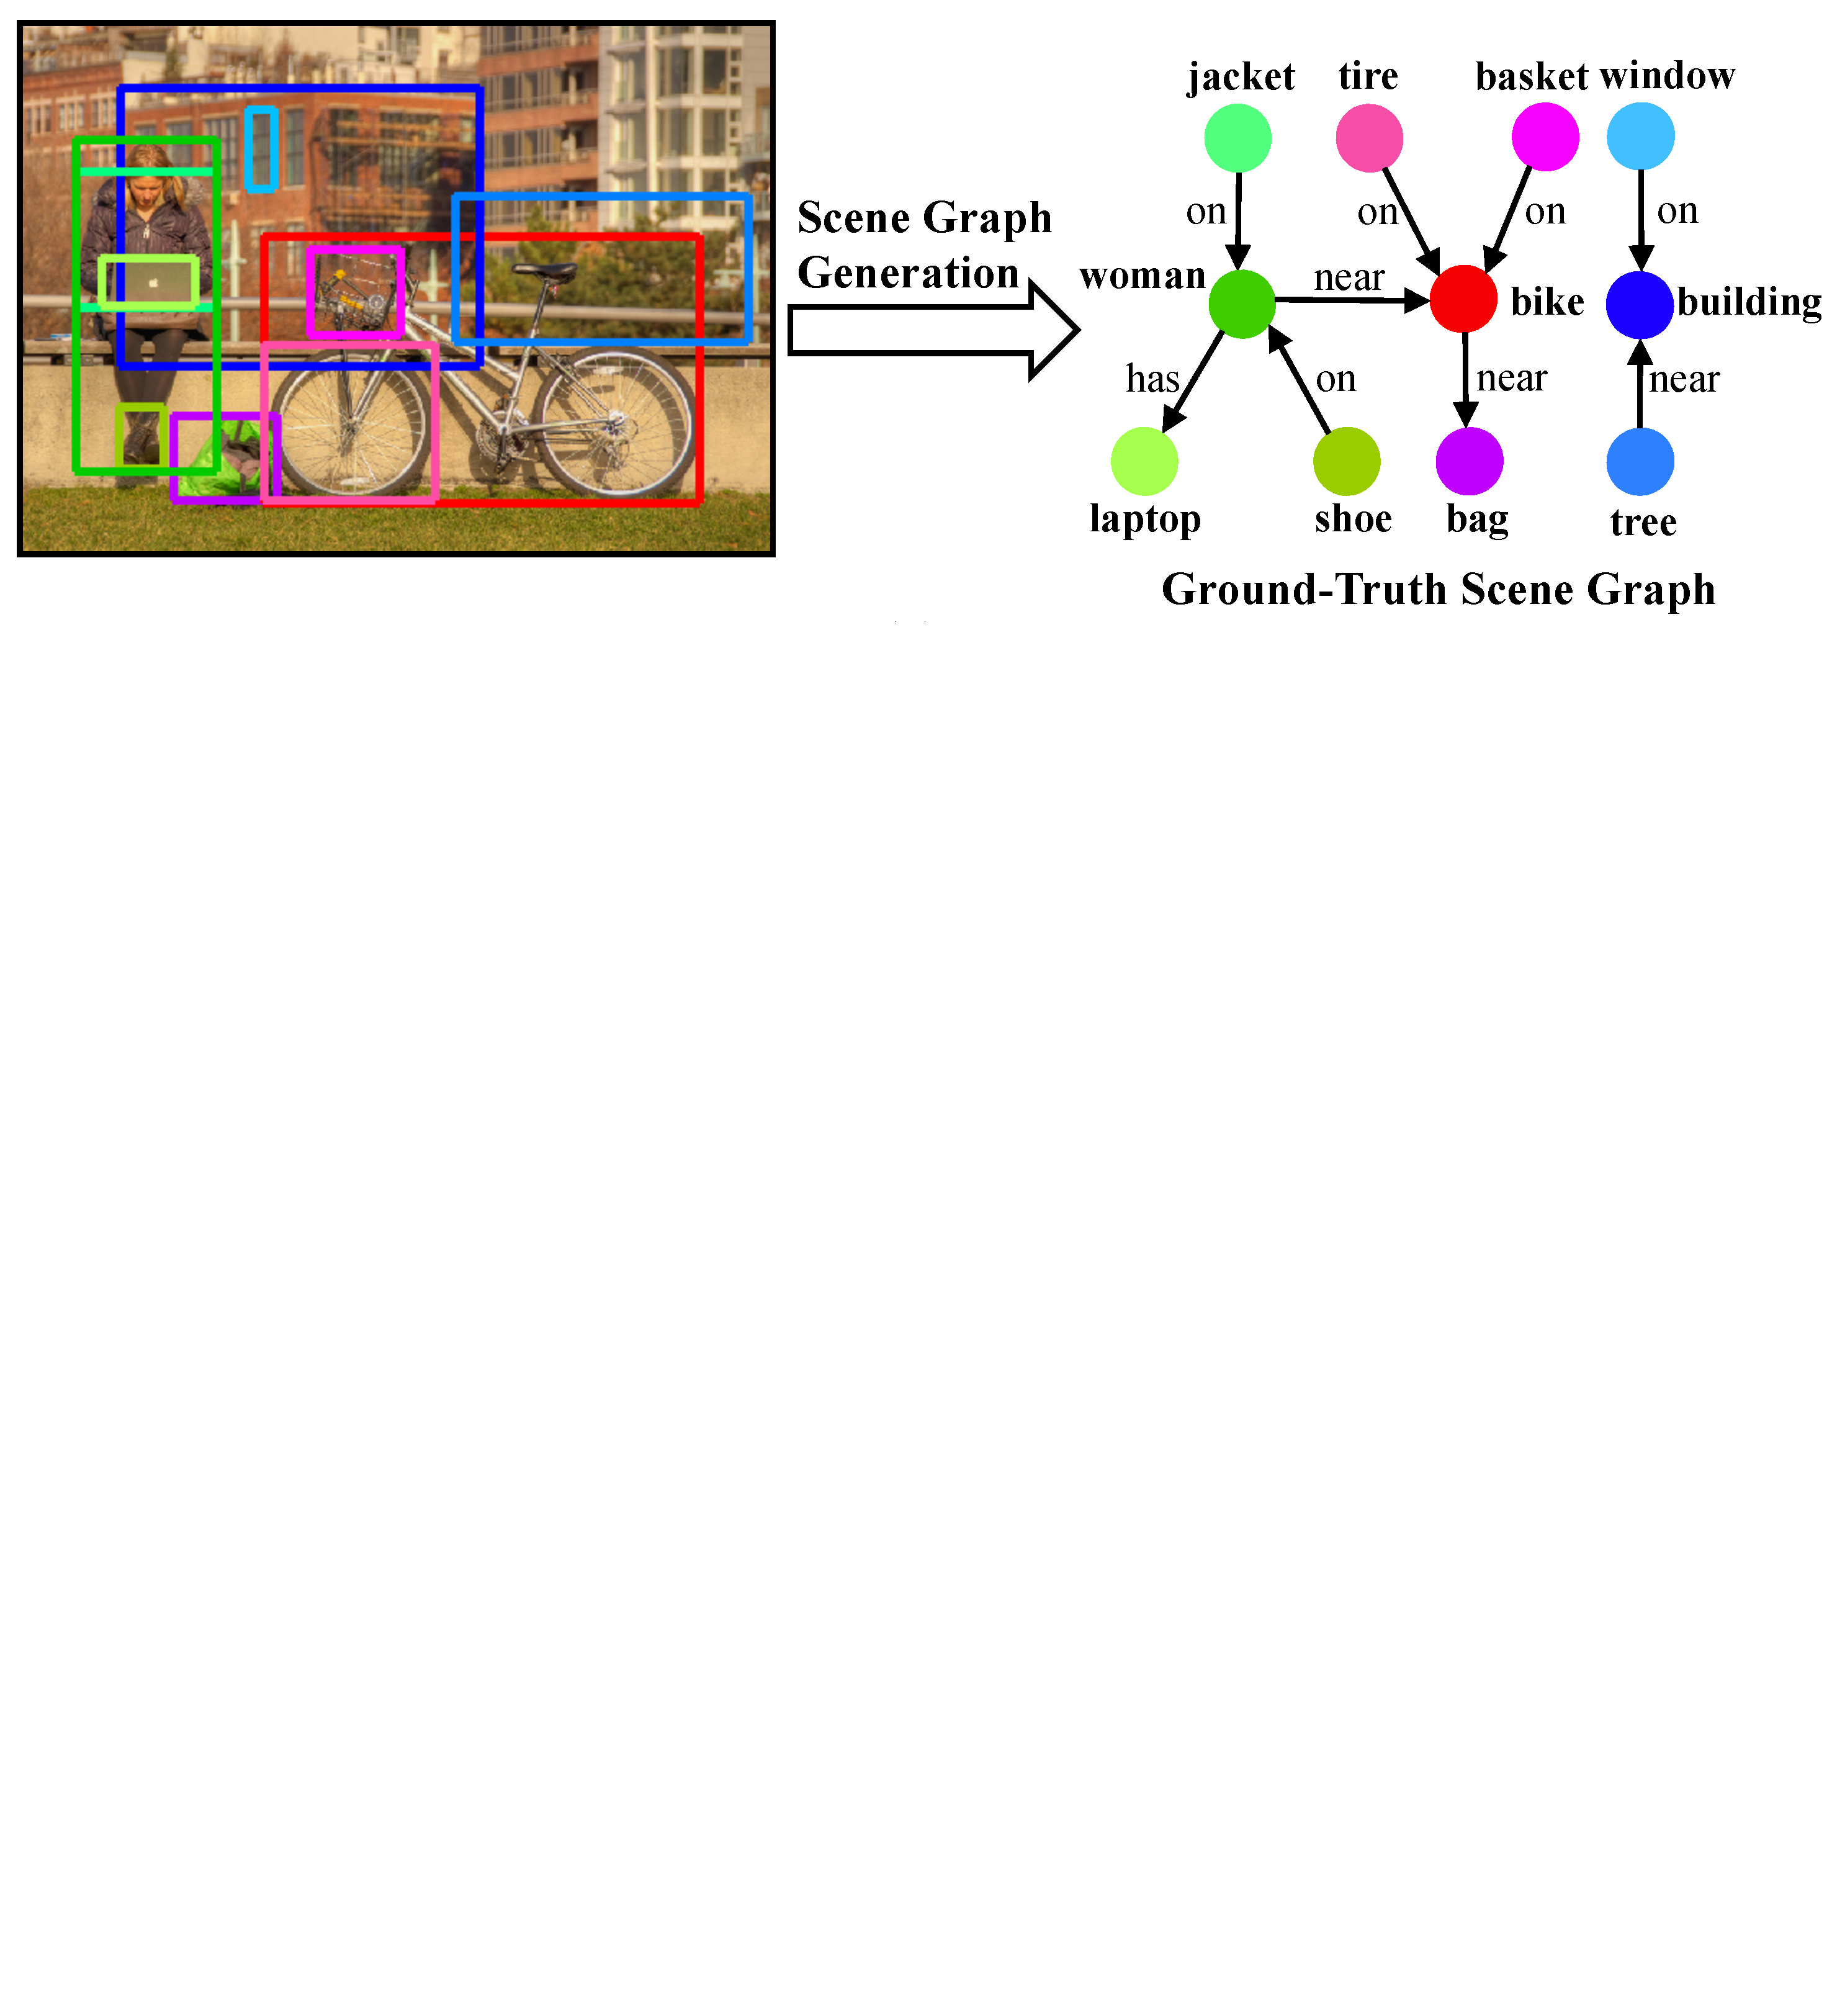
\includegraphics[width=0.95\linewidth]{chapter4/res/sgg.pdf}
    \caption{一个图像视觉场景图生成任务示例}
    \label{ch4:fig:sgg}
\end{figure}


对于图像的视觉场景图生成(Scene Graph Generation, SGG),一个最简单的解决思路是将视觉场景图生成任务分成物体检测和视觉关系检测两个独立的子任务,即先用现有的物体检测器检测物体框,然后预测每个物体框的类别以及两两物体框之间视觉关系的类别~\cite{lu2016visual,zhang2017visual,yang2018shuffle}。然而,这类方法忽略了同一图像中所有物体间的内在联系。通常,这些内在联系往往会提供一些归纳偏置~\cite{divvala2009empirical}(inductive bias)帮助物体或者视觉关系的预测。如图~\ref{ch4:fig:sgg},物体“窗户”(window)和物体“建筑物”(building)常常出现在同一张图像中,“在附近”(near)也是物体“树”(tree)和物体“建筑物”(building)之间最常见的视觉关系。因此,从视觉关系“窗户-在上面-\texttt{?}”或“树-在附近-\texttt{?}”中,很容易推测出“\texttt{?}”是“建筑物”。这些辅助信息已经被广泛地用来提升视觉场景图生成效果~\cite{xu2017scene, dai2017detecting, li2017vip, li2017scene, li2018factorizable, yin2018zoom, jae2018tensorize, zellers2018neural, tang2019learning, gu2019scene, qi2019attentive, wang2019exploring, qian2019video}。具体来说,这些方法都是通过借助条件随机场~\cite{zheng2015conditional}(Conditional Random Field, CRF)来建模所有节点和边的联合分布,然后通过信息传递机制来更新节点和边的特征~\cite{krahenbuhl2011efficient}。最后,整个模型利用所有节点(物体)和边(视觉关系)分类的交叉熵之和作为损失函数进行参数优化。


\begin{figure}[htbp]
    \centering
    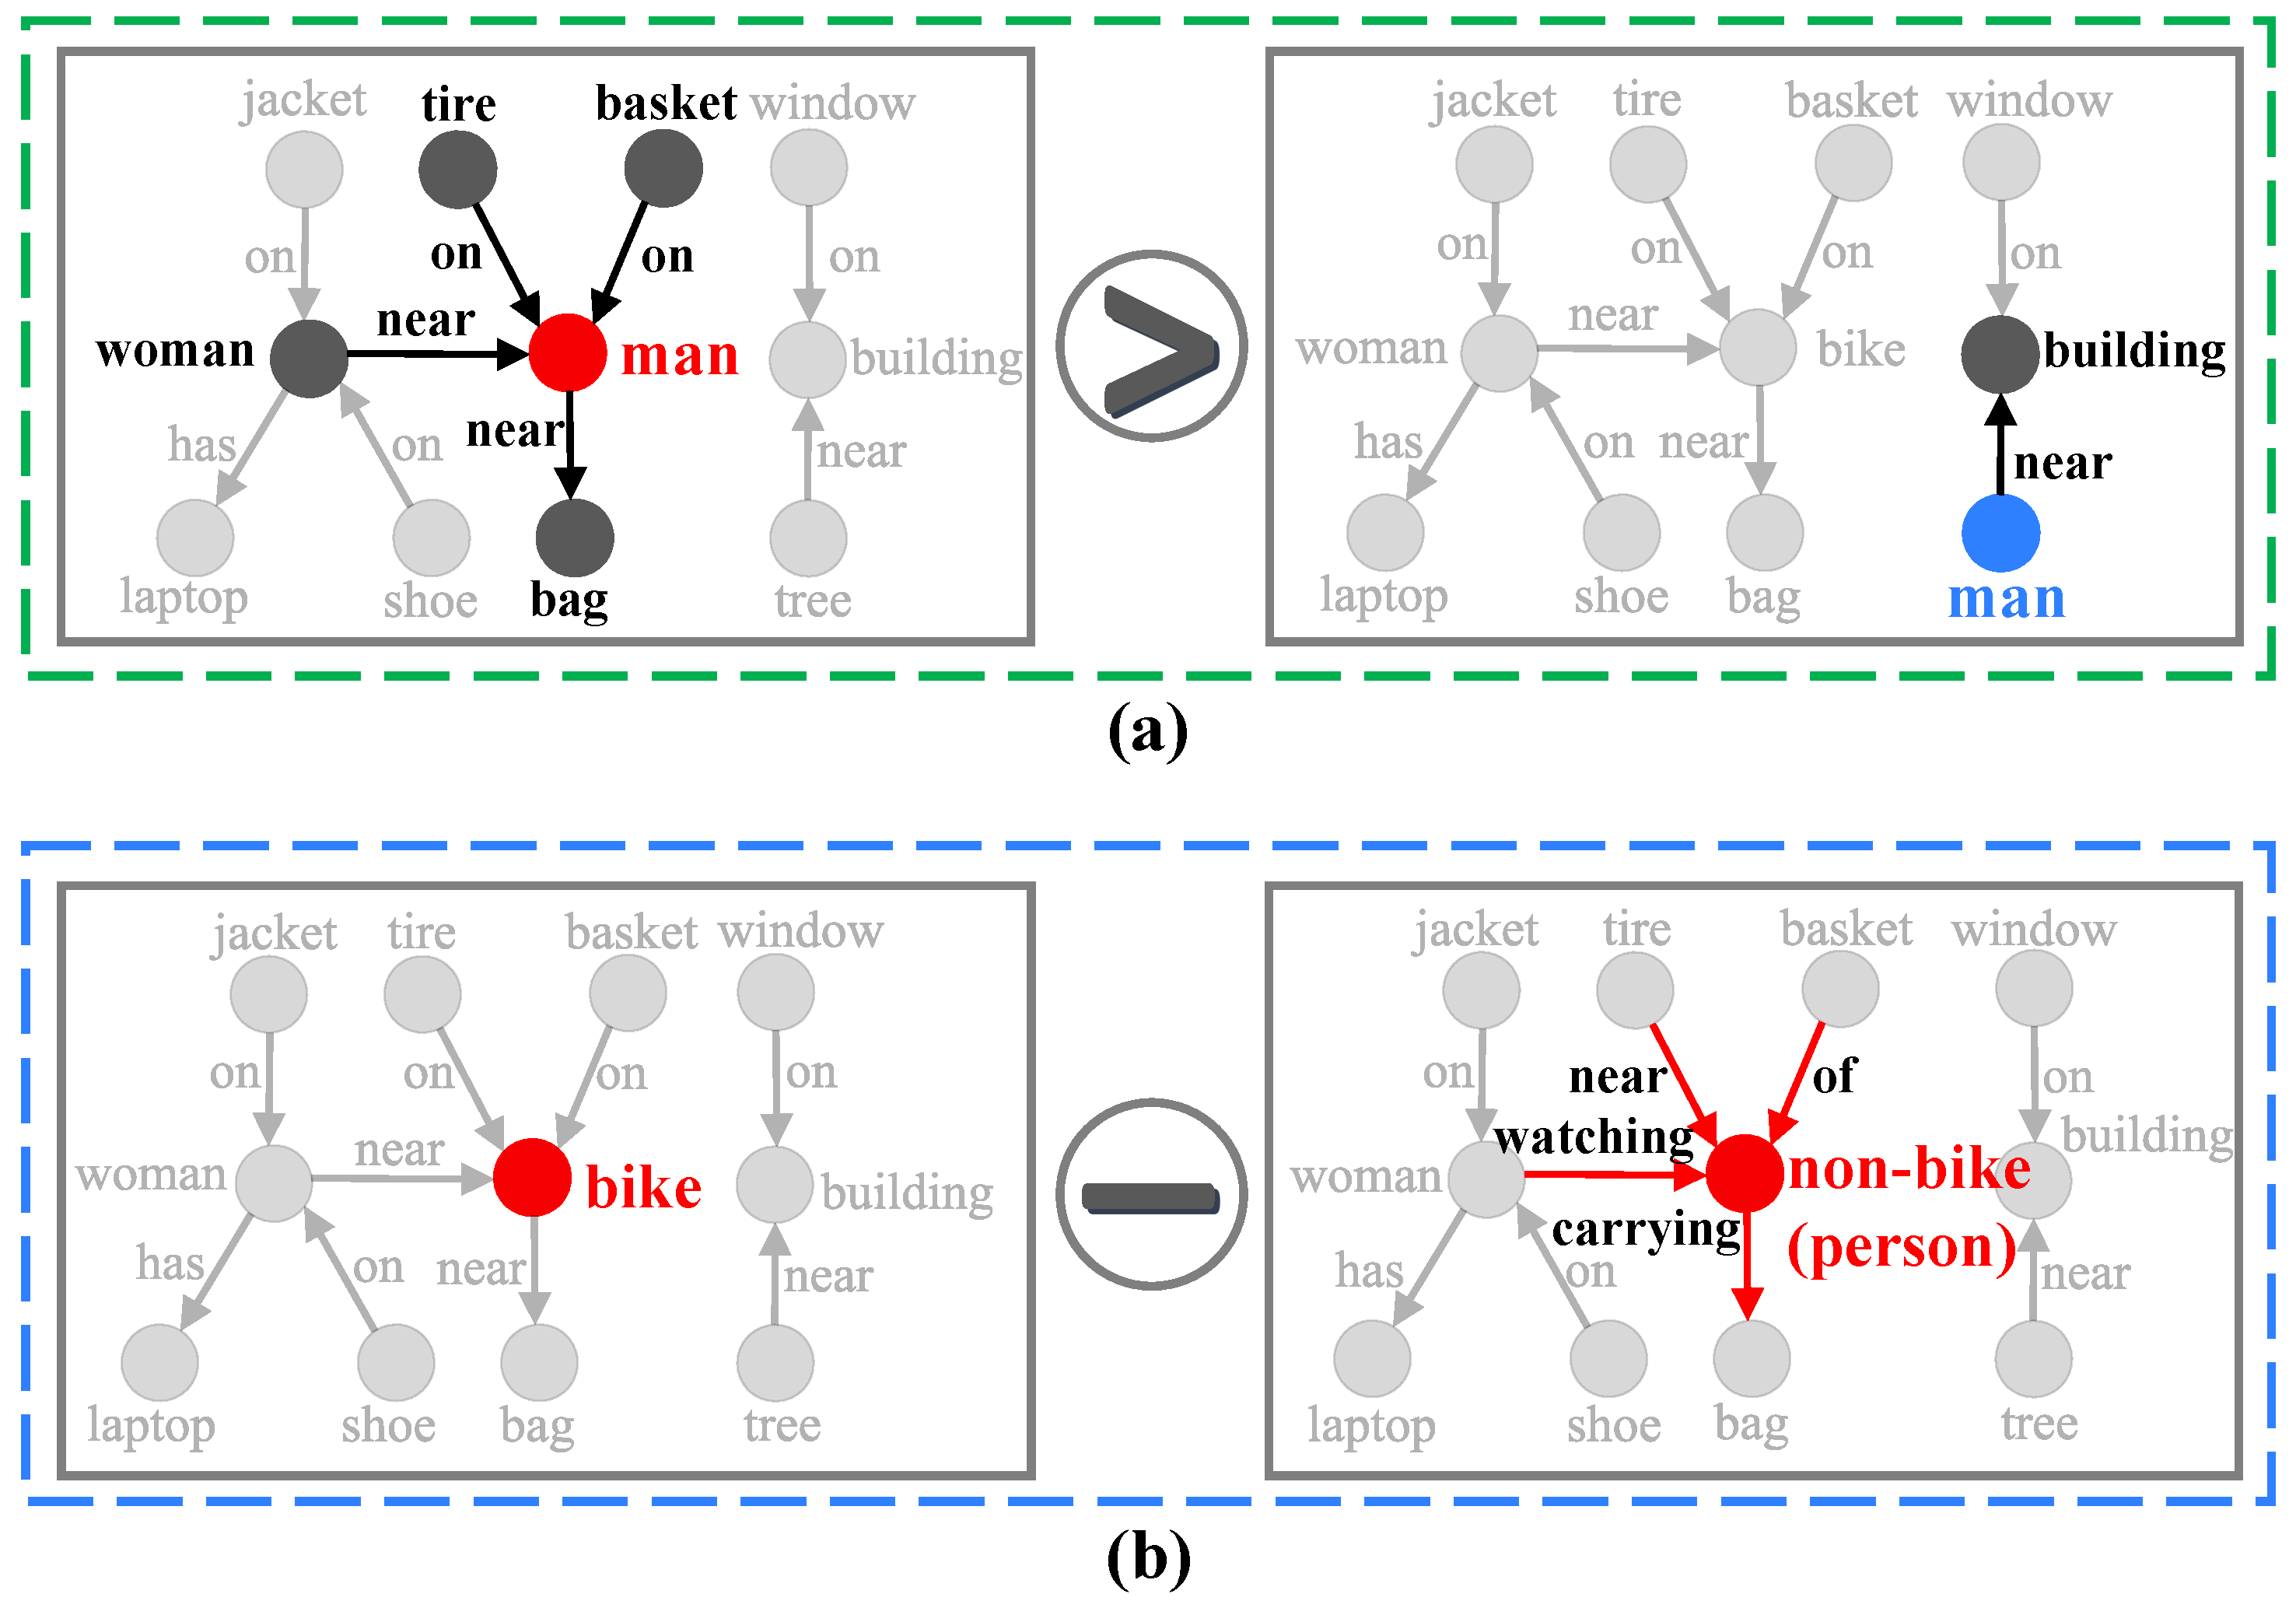
\includegraphics[width=0.95\linewidth]{chapter4/res/motivation.pdf}
    \caption{视觉场景图生成中优化目标的整体一致性和局部敏感性}
    \label{ch4:fig:motivation}
\end{figure}


现有的视觉场景图生成方法对并没有充分地利用图像中物体和视觉关系之间的内在联系,一个重要的原因是交叉熵之和作为视觉场景图生成的优化目标,不具备\textbf{整体一致性}。所谓的“整体一致性”,意思是所有预测的物体类别和视觉关系类别之间应该整体一致。相反,交叉熵之和将所有的物体和视觉关系看成是相互独立的。如图~\ref{ch4:fig:motivation}(a),如果红色节点和蓝色节点都被错误分成类别“man”,根据目前的损失函数(交叉熵之和),这两种错误情况的损失相同。然而,因为红色节点连接的边远多于蓝色节点,即对红色节点的错误分类将造成更大的损失,因为它会影响更多的视觉关系。因此,我们提出直接用Recall@K~\cite{lu2016visual}或者SPICE~\cite{anderson2016spice}这种场景图的全局评价指标作为优化目标。另外,视觉场景图生成的优化目标还应该具备\textbf{局部敏感性}。所谓的“局部敏感性”,意思是优化目标应该能够感知每个节点类别的预测变化。由于场景图的全局评价指标是一个整体生成质量的评价数值,因此我们需要设计一种机制,可以感知每个节点各自的贡献,进而为每个局部预测提供更加有效的优化梯度。


在本章,我们提出了一种全新的训练方式可以同时满足优化目标的整体一致性和局部敏感性:反事实的多智能体学习(CMAT)。具体来说,我们设计了一种全新的多智能体模型,其中将每个物体框看成是一个智能体。每个智能体的动作就是物体类别,智能体之间可以进行通信进而提升智能体的特征表达。在多轮的智能体通信之后,我们利用一个视觉关系预测模型来得到智能体之间的视觉关系。通过与人工标注的场景图对比,得到一个全局的奖励。

为了整体一致性,我们直接将视觉场景图的评价指标(如:Recall@K或SPICE)作为全局奖励,并且使用策略梯度的方式进行参数优化~\cite{sutton2000policy}。从多智能体强化学习~\cite{tampuu2017multiagent,lowe2017multi}(Multi-Agent Reinforcement Learning, MARL)的观点来看,尤其是演员-评论家方法~\cite{lowe2017multi}(actor-critic),CMAT中视觉关系模型可以看成是\textbf{评论家}(critic),而物体类别分类模型可以看成是策略网络。为了局部敏感性,对于每个智能体,我们从全局奖励中减去一个反事实基准~\cite{foerster2018counterfactual}。这个反事实基准模型通过改变目标智能体的预测类别同时固定其他智能体的预测类别,从而得到目标智能体的局部贡献。如图~\ref{ch4:fig:motivation}(b)所示,为了得到红色节点预测为“自行车”(bike)的贡献,我们可以固定其他节点的预测,而将红色节点的预测替换成其他的“非自行车”类。进而可以计算出这种\textbf{反事实}的替换对整体的场景图生成效果带来多大的影响。

为了更好的编码物体之间的内在联系,我们还设计了一种更加有效的智能体通信模型。相比于现有的信息传递机制~\cite{xu2017scene, li2017scene, jae2018tensorize, li2017vip, yin2018zoom, li2018factorizable},我们没有将视觉关系也看成节点。通过这个设计,我们可以将智能体通信与视觉关系预测两个任务分离出来,让前者关注如何编码物体间内在联系,后者作为评论家提供全局奖励引导网络的优化。

我们在目前最大的图像视觉场景图生成数据集Visual Genome(VG)上对CMAT的性能进行了验证。通过大量的对比实验,我们在通用的三个标准实验设定下都可以达到目前最好的效果。

本章主要有三个贡献:
\begin{asparaenum}

\item 我们提出了一种全新的图像视觉场景图生成的优化方式:反事实的多智能体学习(CMAT)。据我们了解,这是第一个将图像场景图生成任务构思成一个多智能体协同合作的问题,使得优化目标满足整体一致性要求。

\item 我们设计了一个全新的反事实基准模型,可以使得多智能体策略梯度算法的优化目标具备局部敏感性。

\item 我们设计了一个有效的多智能体通信模型,有效地将智能体通信与视觉关系预测两个任务分离出来。

\end{asparaenum}


\section{反事实的多智能体学习}

\section{实验设置与性能对比}
\subsection{图像场景图生成数据集与实验设定}

\noindent{\kaishu{图像场景图生成数据集}}:我们使用目前最大的场景图数据集Visual Genome(VG) ~\cite{krishna2017visual}。为了与现有工作能够公平地进行比较,我们采用与现有工作相同的数据集划分和预处理~\cite{xu2017scene, zellers2018neural, newell2017pixels, yang2018graph, herzig2018mapping}。处理后的图像数据共包含150个物体类别和50个视觉关系类别。每张图像平均有11.5个物体和6.2个视觉关系。整个数据集中,70\%的图像数据当成训练集,30\%的图像数据当成测试集。


\noindent{\kaishu{实验设定}}:参考现有的文献~\cite{xu2017scene, zellers2018neural, jae2018tensorize},我们在三种实验设定下评估场景图生成质量:
\begin{asparaenum}
\item 视觉关系分类(PredCls):给定图像、所有的物体框和物体类别,模型需要预测所有的物体组合的视觉关系;

\item 场景图分类(SGCls):给定图像和所有的物体框,模型需要预测所有物体类别以及所有物体组合的视觉关系;

\item 场景图检测(SGDet):给定图像,模型需要检测物体框、预测所有物体类别以及所有物体组合的视觉关系。
\end{asparaenum}

对于视觉关系中物体框检测来说,需要主语(subject)和宾语(object)与真实准确物体框的交并比(IoU)均大于0.5。按照惯例,我们使用Recall@20(R@20)、Recall(R@50)和Recall(R@100)作为场景图生成质量的评价指标。


\subsection{实验细节}


\noindent{\kaishu{物体检测器}}:为了公平地与现有工作进行对比,我们采用了与~\cite{zellers2018neural}相同的物体检测器。具体来说,它是以VGG网络~\cite{simonyan2015very}为主干网络,然后锚框的大小和长宽比与YOLO-9000~\cite{redmon2017yolo9000}设置一样, 然后用RoIAlign~\cite{he2017mask}代替RoIPooling。


\noindent{\kaishu{训练细节}}:我们参照之前的策略梯度的工作,将整个训练过程分成两个阶段,并且先使用监督训练对模型进行参数初始化。在监督训练过程中,我们将RoIAlign层之前的参数都固定住,


\noindent{\kaishu{速度与正确率的权衡}}:在策略梯度的训练过程中,完整的反事实评论家的计算需要对所有可能的物体类别进行加权,通常需要非常多的时间(如:对于64个智能体,每个智能体共有151种物体类别选择,则需要超过9600次($\approx 151 \times 64$)的评估计算)。幸运的是,我们注意到只有极少数的类别有较大的预测概率。为了速度与正确率之间的权衡,我们只对背景(background)和预测概率最高的两种类别进行求和来对所有的类别进行近似。在我们的实验中,这样的实验设定可以把速度提升70倍,同时维持相同的实验效果。


\noindent{\kaishu{SGDet的后处理}}: 对于场景图生成任务(SGDet),为了与之前的工作~\cite{zellers2018neural,zhang2019graphical}公平地进行对比,我们采用相同的后处理操作。具体来说,在对每个RoI预测出物体所有类别的概率分布之后,我们对每个类别使用一次非极大值抑制来确定最终的物体类别,以及对应类别的位移偏置。在我们的实验中,非极大值抑制的IoU阈值设置为0.5。


\subsection{视觉场景图生成性能分析}

%%%%%%%%%%%%%%%%% reward choice %%%%%%%%%%%%%%
\begin{table}
\begin{center}
\scalebox{0.95}{
    \begin{tabular}{|l|l ccc|}
    \hline
    & & XE & R@20 & SPICE  \\
    \hline
    \multirow{2}{*}{SGCls} & R@20 & 34.08 & \textbf{35.93} & 35.27  \\
    & SPICE & 15.39 & \textbf{16.01} & 15.90 \\
    \hline
    \multirow{2}{*}{SGDet} & R@20 & 16.23 & \textbf{16.53} & 16.51  \\
    & SPICE & 7.48 & \textbf{7.66} & 7.64  \\
    \hline
    \end{tabular}
}
\end{center}
\caption{xx}
\label{xx}
\end{table}
%%%%%%%%%%%%%%%%%%%%%%%%%%%%%%%%%%%%%%%%%%%%%%%%%%%%


%%%%%%%%%%%%%%%%% baseline types %%%%%%%%%%%%%%
\begin{table}
\begin{center}
\scalebox{0.95}{
    \begin{tabular}{|l|l cccc|}
    \hline
    & & XE & MA & SC & CF  \\
    \hline
    \multirow{3}{*}{SGCls} & R@20 & 34.08 & 34.76 & 34.68 & \textbf{35.93} \\
    & R@50 & 36.90 & 37.58 & 37.54 & \textbf{39.00} \\
    & R@100 & 37.61 & 38.29 & 38.25 & \textbf{39.75} \\
    \hline
    \multirow{3}{*}{SGDet} & R@20 & 16.23 & 16.07 & 16.37 & \textbf{16.53} \\
    & R@50 & 20.62 & 20.41 & 20.82 & \textbf{20.95} \\
    & R@100 & 23.24 & 23.02 & 23.41 & \textbf{23.62} \\
    \hline
    \end{tabular}
}
\end{center}
\caption{xx}
\label{xx}
\end{table}
%%%%%%%%%%%%%%%%%%%%%%%%%%%%%%%%%%%%%%%%%%%%%%%%%%%%



%%%%%%%%%%%%%%%%% communication steps %%%%%%%%%%%%%%
\begin{table}
\begin{center}
\scalebox{0.95}{
    \begin{tabular}{|l|l cccc|}
    \hline
    & & 2-step & 3-step & 4-step & 5-step  \\
    \hline
    \multirow{3}{*}{SGCls} & R@20 & 35.09 & 35.25 & 35.40 & \textbf{35.93} \\
    & R@50 & 37.95  & 38.19 & 38.37 & \textbf{39.00} \\
    & R@100 & 38.67 & 38.91 & 39.09 & \textbf{39.75} \\
    \hline
    \multirow{3}{*}{SGDet} & R@20 & 16.35 & 16.43 & 16.47 & \textbf{16.53} \\
    & R@50 & 20.89 & 20.88 & 20.92 & \textbf{20.95} \\
    & R@100 & 23.49 & 23.50 & 23.54 & \textbf{23.62} \\
    \hline
    \end{tabular}
}
\end{center}
\caption{xx}
\label{xx}
\end{table}
%%%%%%%%%%%%%%%%%%%%%%%%%%%%%%%%%%%%%%%%%%%%%%%%%%%%



\subsection{视觉场景图生成性能对比}
本节将本章方法与目前最先进的视觉场景图生成算法进行对比。这些方法主要可以分为两大类:(1)VRD~\cite{lu2016visual}, AED~\cite{newell2017pixels}, FREQ~\cite{zellers2018neural}。这类方法都是将视觉场景图生成任务分解成物体检测和视觉关系检测两个独立的任务。(2)MSDN~\cite{li2017scene}, IMP~\cite{xu2017scene}, TFR~\cite{jae2018tensorize}, MOTIFS~\cite{zellers2018neural}, G-RCNN~\cite{yang2018graph}, GPI~\cite{herzig2018mapping}, KER~\cite{chen2019knowledge}。这类方法利用信息传递机制来编码物体间的内在联系。所有的方法都是利用交叉熵之和作为模型的损失函数。


%%%%%%%%%%%%%%%%%%%%%%% SOTA %%%%%%%%%%%%%%%%%%%%%%%%%%
\begin{table*}
\small
\begin{center}
\scalebox{0.95}{
\begin{tabular}{|l|l|ccc|ccc|ccc|}
\hline
& & \multicolumn{3}{c|}{SGDet} & \multicolumn{3}{c|}{SGCls} & \multicolumn{3}{c|}{PredCls} \\
& Model & R@20 & R@50 & R@100  & R@20 & R@50 & R@100 & R@20 & R@50 & R@100 \\ 
\hline\hline
\parbox[t]{2mm}{\multirow{12}{*}{\rotatebox[origin=c]{90}{Graph Constraint}}} & VRD & - & 0.3 & 0.5 & - & 11.8 & 14.1 & - & 27.9 & 35.0 \\
& IMP & - & 3.4 & 4.2 & - & 21.7 & 24.4 & - & 44.8 & 53.0  \\
& MSDN & - & 7.0 & 9.1 & - & 27.6 & 29.9 & - & 53.2 & 57.9 \\
& AED & 6.5 & 8.1 & 8.2 & 18.2 & 21.8 & 22.6 & 47.9 & 54.1 & 55.4 \\
& FREQ+ & 20.1 & 26.2 & 30.1 & 29.3 & 32.3 & 32.9 & 53.6 & 60.6 & 62.2 \\
& IMP+ & 14.6 & 20.7 & 24.5 & 31.7 & 34.6 & 35.4 & 52.7 & 59.3 & 61.3 \\
& TFR & 3.4 & 4.8 & 6.0 & 19.6 & 24.3 & 26.6 & 40.1 & 51.9 & 58.3 \\
& MOTIFS & 21.4 & 27.2 & 30.3 & 32.9 & 35.8 & 36.5 & 58.5 & 65.2 & 67.1 \\
& G-RCNN & - & 11.4 & 13.7 & - & 29.6 & 31.6 & - & 54.2 & 59.1 \\
& GPI & - & - & - & - & 36.5 & 38.8 & - & 65.1 & 66.9 \\
& KER & - & 27.1 & 29.8 & - & 36.7 & 37.4 & - & 65.8 & 67.6 \\
& \textbf{CMAT} & \textbf{22.1} & \textbf{27.9} & \textbf{31.2} & \textbf{35.9} & \textbf{39.0} & \textbf{39.8} & \textbf{60.2} & \textbf{66.4} & \textbf{68.1} \\
\hline
\parbox[t]{2mm}{\multirow{6}{*}{\rotatebox[origin=c]{90}{No Constraint}}} & AED & - & 9.7 & 11.3 & - & 26.5 & 30.0 & - & 68.0 & 75.2 \\
& IMP+ & - & 22.0 & 27.4 & - & 43.4 & 47.2 & - & 75.2 & 83.6  \\
& FREQ+ & - & 28.6 & 34.4 & - & 39.0 & 43.4 & - & 75.7 & 82.9  \\
& MOTIFS & 22.8 & 30.5 & 35.8 & 37.6 & 44.5 & 47.7 & 66.6 & 81.1 & 88.3  \\
& KER & - & 30.9 & 35.8 & - & 45.9 & 49.0 & - & 81.9 & 88.9  \\
& \textbf{CMAT} & \textbf{23.7} & \textbf{31.6} & \textbf{36.8} & \textbf{41.0} & \textbf{48.6} & \textbf{52.0} & \textbf{68.9} & \textbf{83.2} & \textbf{90.1} \\
\hline
\end{tabular}
}
\end{center}
\caption{不同场景图生成方法在VG数据集上的性能对比}
\label{ch4:tab:sota}
\end{table*}
%%%%%%%%%%%%%%%%%%%%%%%%%%%%%%%%%%%%%%%%%%%%%%%%%%%%

\textbf{定量性能分析}:表~\ref{ch4:tab:sota}展示了不同场景图生成方法在VG数据集上的实验结果。由表~\ref{ch4:tab:sota}可以看出,CMAT在所有的评估指标下都达到了最好的性能。尤其值得注意的是,CMAT在场景图分类(SGCls)任务中可以显著提升实验效果(即:在有图限制~\cite{zellers2018neural}和没有图限制的条件下可以分别提升3.4\%和4.3\%)。这也刚好符合我们的设计动机,通过将预测物体类别看成智能体的动作选择,较好地提升物体的类别预测准确率。另一方面,实验结果也表明反事实多智能体学习可以显著的提升场景图生成任务的性能。对于视觉关系分类任务(PredCls),即使我们使用的视觉关系分类模型非常简单,我们仍然可以达到最好的实验性能。这说明CMAT中,视觉关系分类模型的输入已经更好地编码了智能体的内部状态。另外,CMAT模型可以兼容任何效果更好的视觉关系分类模型。对于场景图检测任务(SGDet),CMAT的提升没有场景图分类任务明显,原因可以来自于物体检测框的准确率特别高。


\begin{figure}[htbp]
    \centering
    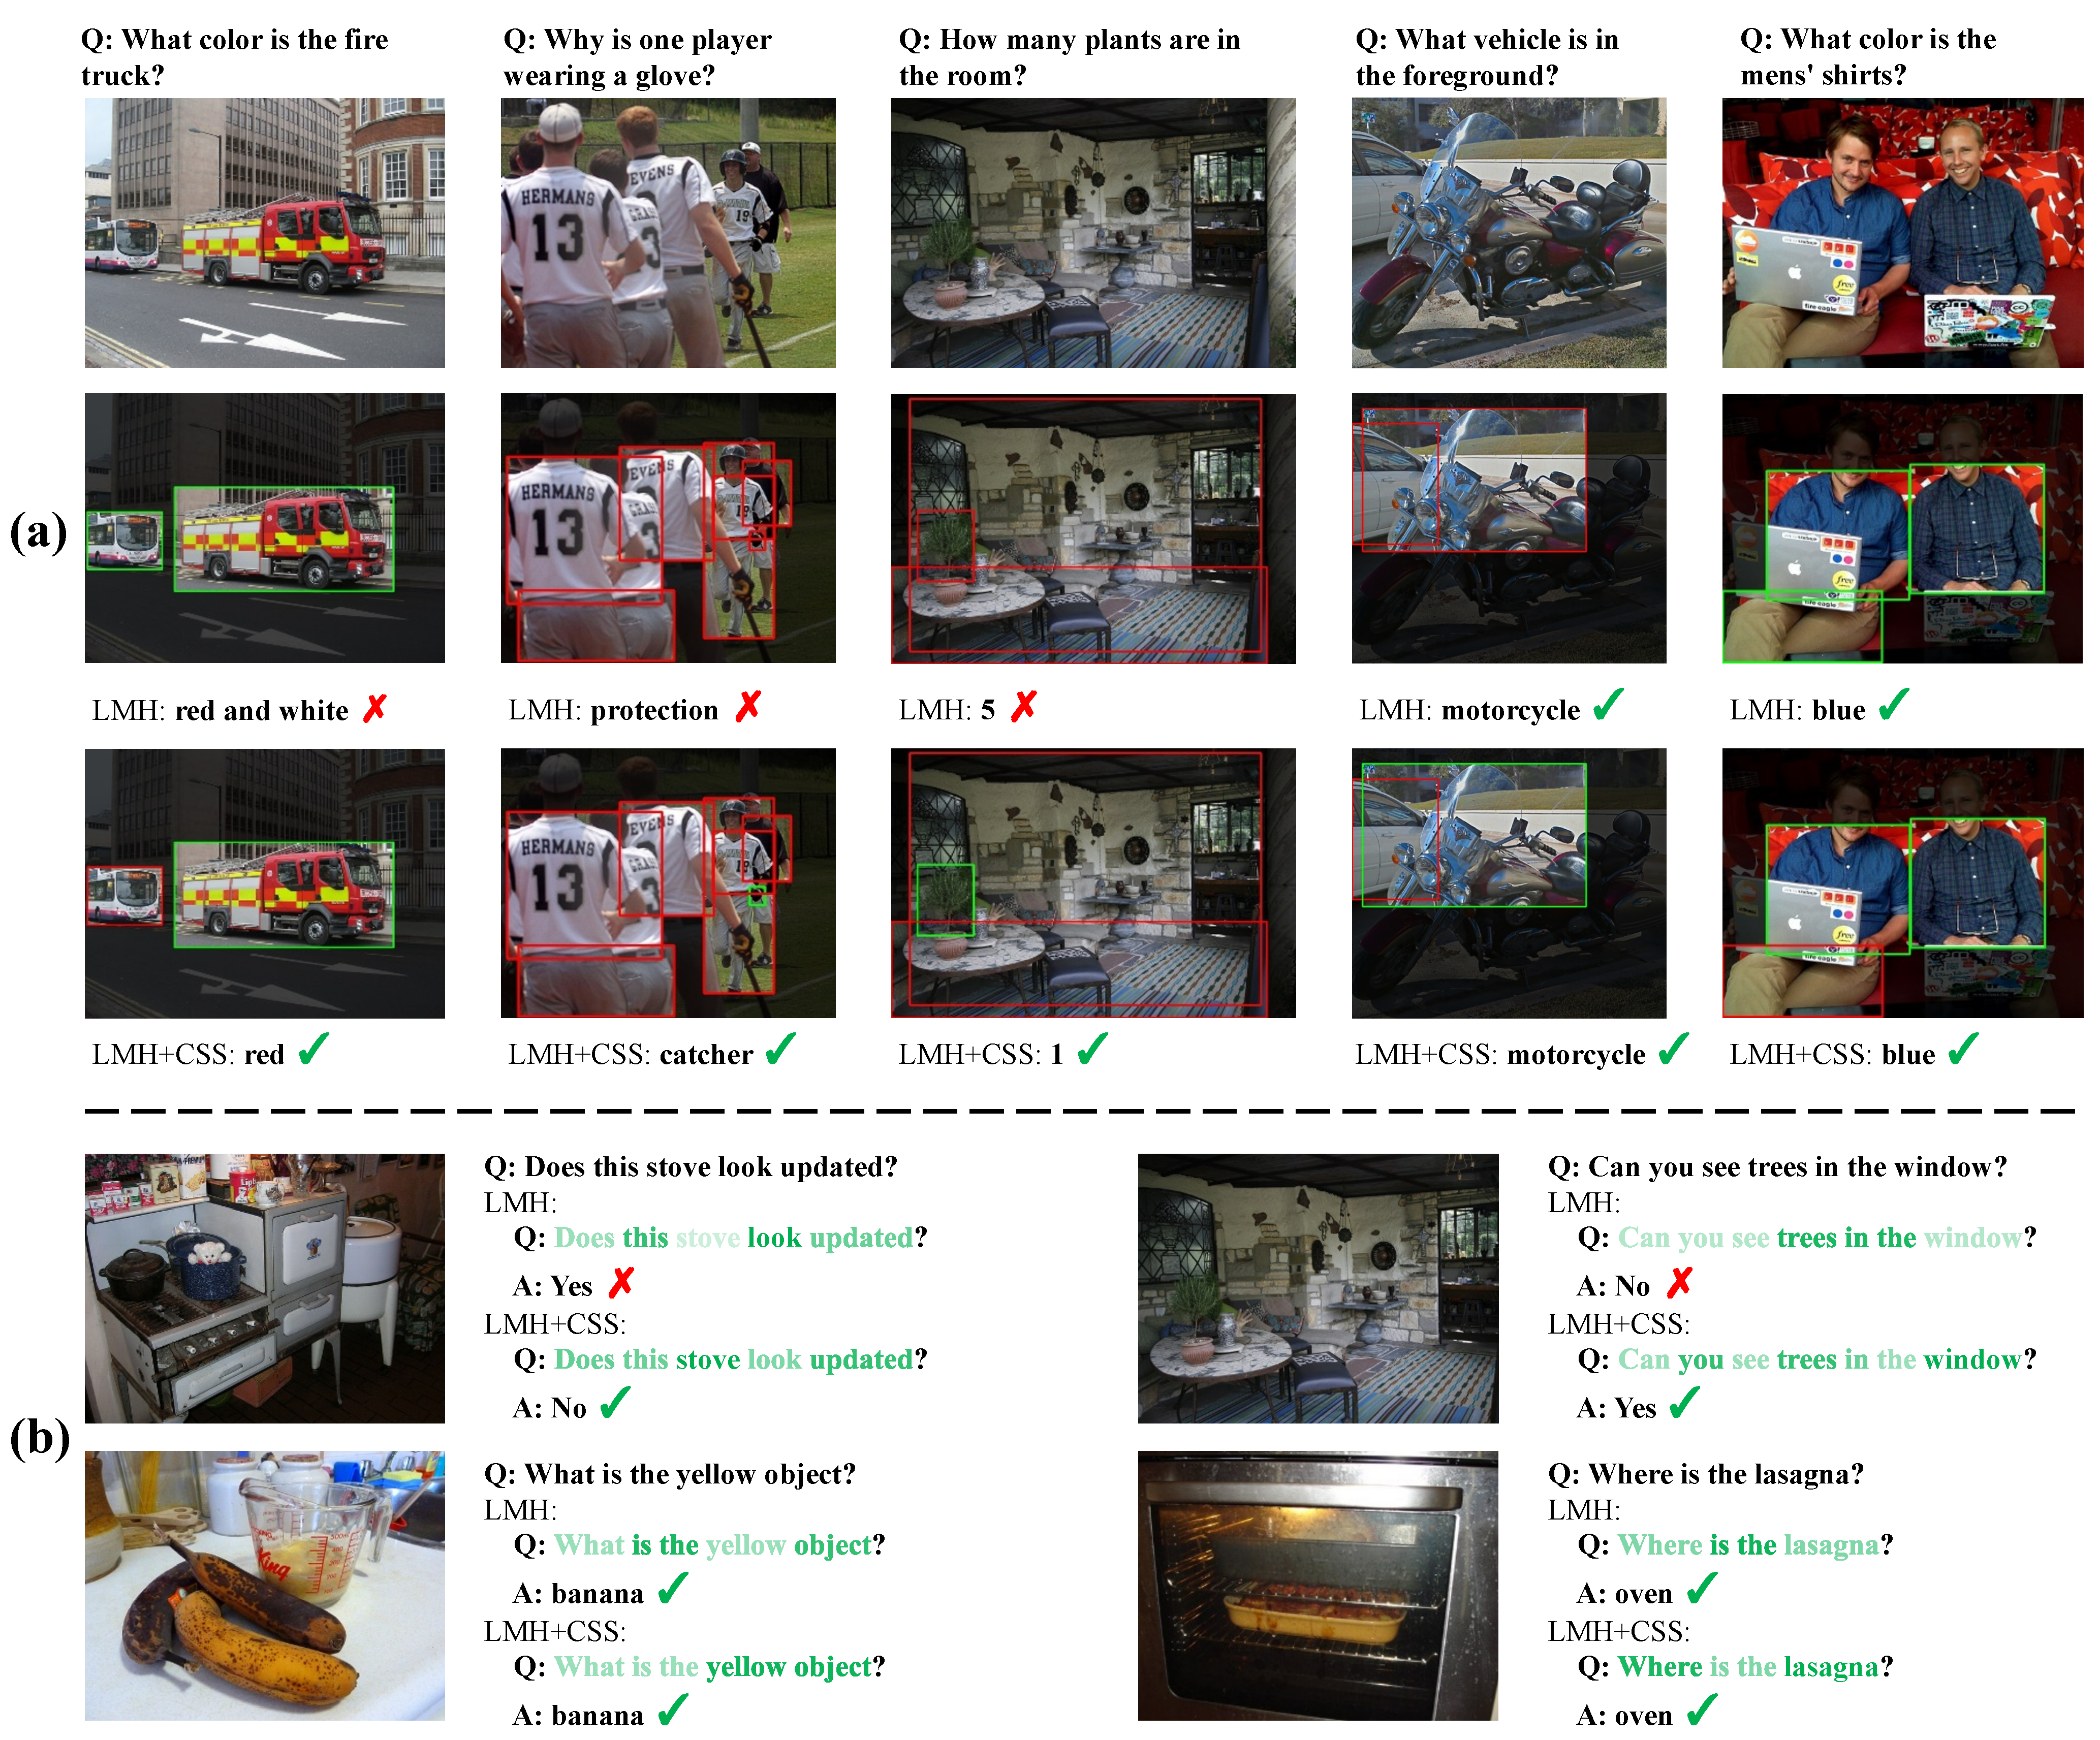
\includegraphics[width=0.95\linewidth]{chapter4/res/visualization.pdf}
    \caption{CMAT和MOTIFS在数据集VG上的场景图生成结果对比}
    \label{ch4:fig:visualization}
\end{figure}

\textbf{定性性能对比}:图~\ref{ch4:fig:visualization}展示了CMAT和MOTIFS在数据集VG上的场景图生成结果。由前两排结果看出可以看出,CMAT很少漏掉一些重要的节点,如“laptop”、“surfboard”等。因为CMAT的优化目标满足整体一致性。从第三排结果可以看出,CMAT的错误主要是检测出比MOTIFS更多的未标注的视觉关系(蓝色边)。由于目前使用的评价指标主要是Recall@K,它主要是基于所有标注的三元组序列的排序结果。因此,如果检测出更多的未标注的正样本,反而得到更低的值。




\section{本章小结}